\chapter{Fundamentação Teórica}
\label{cap2}



\section{Jogos Eletrônicos}



O primeiro sistema de entretenimento interativo foi construido em 1947, utilizando como base de exibição um tubo de raios catódicos, criado por Thomas Goldsmith Jr. e Estle Ray Mann.
%
Essa criação foi patenteada em janeiro de 1948, datando então o inicio dos jogos eletrônicos~\cite{Adams2014Jan, patents1947Jan}.



O jogo eletrônico, ou entretenimento interativo, é uma atividade intelectual que integra um sistema de regras, na qual utiliza tal sistema a fim de definir seus objetivos ou pontuação por meio de um computador a fim de dispertar alguma emoção ao jogador~\cite{video_game_technologies}.
%
Os jogos eletrônicos são aplicações convencionais, que executam sobre algum sistema operacional ou hardware apropriado a este fim.
%
O sistema operacional, hardware ou base de execução da aplicação gráfica define a sua plataforma, \textit{e. g.,} Linux, Windows, PS4, XBox, Web~\cite{adams_1208533}.



Inicialmente os jogos eram implementados de forma simples por conta da limitação das plataformas dos anos 80.
%
As implementações de jogos para videogames eram desenhadas diretamente para algum hardware proprietário, sem sistema operacional, por muitas vezes sem utilizar comunicação por rede ou memória de disco~\cite{adams_1208533}.
%
Já os jogos de computadores utilizando algum serviço online eram inviabilizados pelo custo de manutenção de tais serviços e pela baixa demanda de jogadores~\cite{adams_1208533}.
%
Na década de 80, o videogame Atari foi uma plataforma popular, vendendo 30.000 cópias em seu lançamento contra apenas 2.000 cópias do seu concorrente Intellivision~\cite{atari_age}. A sua especificação era:



\begin{itemize}
  \item \ac{cpu} com 1.19 \ac{mhz}
  \item Processador de audio e vídeo dedicado \ac{tia}, permitindo a alteração de 40 x 192 pixels a cada frame usando a tecnologia \ac{ntsc} e 2 canais de som monofônico com 4 bits de intonação e 1 bit de volume.
  \item 128 bytes de memória \ac{RAM}, podendo ser expandido com o cartucho.
  \item Os cartuchos podem ter, no máximo, 4 kB de capacidade.
\end{itemize}



Com o crescente recurso computacional disponível em computadores pessoais e videogames após os anos 90, desenvolvedores criaram novos estilos de jogos que utilizavam a comunicação entre computadores.
%
Jogos como Habitat\footnote{Habitat: \url{http://www.mobygames.com/game/c64/habitat/credits}}, Tibia\footnote{Tibia: \url{http://www.tibia.com/}} e Runescape\footnote{Runescape: \url{https://www.runescape.com}} começam a utilizar, como requisito obrigatório do jogo, a conexão com a Internet.
%
Tais títulos tornaram-se jogos populares do gênero \ac{mmo}, deixando de ser somente aplicações locais para ser clientes de um serviço arquitetado na Internet~\cite{adams_1208533, Adams2014Jan}.



\subsection{Árvore de gêneros de jogos eletrônicos}



\begin{figure}[htb!]
\caption{Árvore de gêneros simplificada.}
\label{fig:generos}
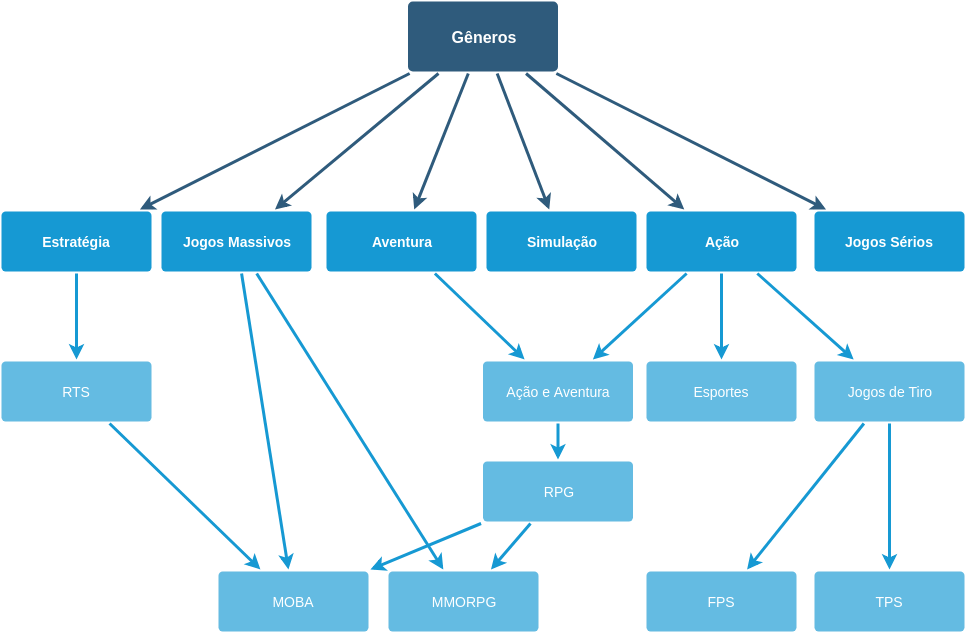
\includegraphics[height=9cm]{img/cap2/generos.png}
\centering

Adaptado de:~\cite{adams_1208533}
\end{figure}



Um gênero de jogo eletrônico é uma categoria específica para agrupar estilos de jogabilidade parecidos.
%
Porém, gêneros não definem definitivamente o conteúdo expresso em algum título, mas sim um desafio comum presente no título analisado~\cite{adams_1208533, video_game_technologies}.
%
Cada gênero de jogo contém várias variações, para uma melhor classificação.
%
A árvore pode ser visualizada pelo diagrama na figura \ref{fig:generos}.



\begin{itemize}
  \item Estratégia: Jogos de estratégia são focados em uma jogabilidade que exija habilidades de raciocínio e/ou gerenciamento de recurso. Neste gênero, o jogador tem uma boa visualização do mundo, controlando indiretamente as suas tropas disponíveis~\cite{rollings2003andrew}. É comum encontrar jogos que disponibilizam algum modo de competição entre jogadores em uma rede local ou via Internet.
    \begin{itemize}
      \item \ac{rts}: Esse subgênero indica que as jogadas dos jogadores não são atômicas. Esse gênero tornou-se popular com grantes torneios do jogo StarCraft II\footnote{StarCraft II: \url{https://starcraft2.com/}} nos anos 2010 e 2011.
    \end{itemize}
  \item Jogos Massivos: Esse gênero de jogo preza pela interação com outros jogadores em um mundo compartilhado. SecondLife\footnote{SecondLife: \url{https://www.secondlife.com/}} é um jogo focado na interação social, com artifícios de comércio e relacionamentos em um mundo fictício criado pela comunidade~\cite{tecmundo_secondlife}.
    \begin{itemize}
      \item \ac{moba}: Este jogo coloca um número fixo de jogadores separados em dois times, no qual o time com maior estratégia de posicionamento e gerenciamento de recursos em equipe ganha a partida. Jogos \ac{moba} perdem o posicionamento de jogos \ac{rpg}, deixando de lado a interpretação e contextualização de um mundo, fixando-se somente em um comate estratégico e momentânio entre as equipes, carregando consigo somente as características de comércio e comunidade dos jogos \ac{mmo}. Tal subgênero é popular por grandes títulos como Dota 2\footnote{Dota 2: \url{http://br.dota2.com/}} e League of Legends\footnote{League of Legends: \url{https://br.leagueoflegends.com/pt/}}. O jogo League of Legends obteve 100 milhões de usuários ativos em 2016~\cite{lol_statista}, além de ter um torneio nacional e mundial~\cite{lol_sportv}.
      \item \ac{mmorpg}: Esse gênero herda características dos gêneros ação e aventura, \ac{rpg}, e \ac{mmo} diretamente. Nesse gênero, o jogo permite interações em um mundo onde outros jogadores também estão jogando, permitindo a interação entre outros jogadores (herdado dos jogos \ac{mmo}), com o mundo (herdado dos jogos de ação e aventura), e com objetivos guiados por \ac{npcs} (herdados de jogos \ac{rpg}). Um título popular para esse gênero é o jogo Word of WarCraft\footnote{Word of WarCraft: \url{https://worldofwarcraft.com/pt-br/}}. Esse gênero será melhor abordado na seção \ref{sec:mmorpg}.
    \end{itemize}
  \item Aventura: Este jogo é caracterizado por desafios envolvendo ações com diversos \ac{npcs} ou com o ambiente. É comum nesses jogos a única interação ser somente por terminal (os primeiros jogos do gênero nos anos 80) ou atualmente somente com mouse e cenários estáticos.
    \begin{itemize}
      \item Ação e Aventura: Esse gênero herda características da categoria de Ação e Aventura. O jogador é imerso em um mundo para iteragir com o ambiente e com \ac{npcs}, além de se preocupar com a movimentação no cenário. Um grande título desse gênero é a série de jogos nomeada The Legend of Zelda\footnote{The Legend of Zelda: \url{https://www.zelda.com/}}.
    \end{itemize}
  \item Simulação: Essa categoria de jogos são desenhados sobre aspéctos reais ou fictícios da realidade. Temas comums nessa super categoria são jogos de construção e gerenciamento, animais de estimação ou vida social e simulação de veículos. Nesses jogos se faz comum partidas geradas proceduralmente contra o computador ou em um conjunto de regras fixo, sem a necessidade da conexão com a Internet.
    \begin{itemize}
      \item Esportes: Essa subcategoria da simulação trata somente da simulação de esportes, onde o(s) time(s) podem ser controlados tanto por uma inteligência artificial quanto por jogadores online. O jogo FIFA\footnote{FIFA: \url{https://www.easports.com/br/fifa}} é um título popular nesse segmento.
    \end{itemize}
  \item Ação: Essa categoria de jogos preza pela habilidade de coordenação motora e reflexos do jogador, para tomar uma atitude a fim de passar seus objetivos no cenário. Nesse gênero os objetivos são passar por uma série de desafios que incluam movimentação e posicionamento de outros objetos no cenário.
    \begin{itemize}
      \item Jogos de Tiro: Em jogos de tiro, o jogador usa um número finito de armas para executar ações a distância. Essa categoria de jogos contém conteúdo de violência, geralmente caracterizado por jogos de 16 anos na classificação indicativa do Brasil~\cite{trindade2018Apr}.
        \begin{itemize}
          \item \ac{fps}: Nessa subcategoria, o jogo utiliza o método de gravação conhecido como \ac{pov}. Nesse método, o modo de exibição do mundo é dado como a visão de um personagem do jogo, onde o personagem não tem visão de sí próprio se não por reflexos~\cite{video_game_technologies}.
          \item \ac{tps}: Diferente dos jogos \ac{fps}, os jogos \ac{tps} utilizam cameras soltas no cenário onde o jogador é visível na cena.
        \end{itemize}
    \end{itemize}
  \item Jogos sérios: Esse gênero de jogo tem como objetivo transmitir um conteúdo educacional. O jogo Sherlock Dengue 8~\cite{sherlock_dengue} é um título desenvolvido com o objetivo de conscientizar os problemas e a prevenção da Dengue no Brasil.
\end{itemize}


\section{Jogos Massivos}
\label{sec:mmorpg}



Jogos \ac{mmorpg} são utilizados como negócio viável e lucrativo, sendo que experiência de jogabilidade na qual o usuário final será submitido é um fator crítico para o sucesso.
%
O mercado de jogos \ac{mmorpg} vem crescendo desde 2012~\cite{new_york_times}, sendo no ano de 2016 um dos mais lucrativos~\cite{statista_2016}.
%
A sua projeção para 2018 é que sejam arrecadados mais de 30 bilhões de dólares americanos com esta categoria de jogos~\cite{statista_2018}, um aumento de 20\% a mais sobre o ano de 2016.



\ac{mmorpg} são jogos de interpretação de papéis massivos, originados dos gêneros \ac{rpg}.
%
A principal característica desse estilo de jogo é a comunicação e representação virtual de um mundo fantasia no qual cada jogador pode interagir com objetos virtuais compartilhados ou tomar ações sobre outros jogadores em tempo real, tendo como principais objetivos a resolução de problemas conforme a sua regra de \textit{design}, o desenvolvimento do personagem e a interação entre os jogadores\cite{video_game_technologies}.
%

Um jogo \ac{mmorpg} é arquitetado em duas partes~\cite{mmo_analytic}:
\begin{itemize}
  \item \textbf{Serviço}: É o macrosserviço que implementa as regras de negócio e requisitos do jogo.
  O serviço disponibiliza uma interface com ações possíveis ao cliente sobre algum protocolo de rede.
  \item \textbf{Cliente}: Cliente é a aplicação que realizará as requisições com a interface do macrosserviço, exibindo o estado de jogo de forma imersiva ao jogador.
\end{itemize}



A maioria dos jogos \ac{mmorpg} disponíveis no mercado estão implementados sobre uma arquitetura que executa sobre diversos servidores\cite{stephenclarkewillson2017}, nos quais o desempenho destes servidores influencia tanto na experiência de jogabilidade do usuário final, quanto no custo de manutenção destes serviços~\cite{1417630}.
%
Em especial, o presente trabalho tratará com maiores detalhes as arquiteturas utilizadas no serviço dessa categoria de jogos.


\section{Arquitetura de Serviços MMORPG}

Lorem ipsum dolor sit amet, consectetur adipisicing elit, sed do eiusmod tempor incididunt ut labore et dolore magna aliqua. Ut enim ad minim veniam, quis nostrud exercitation ullamco laboris nisi ut aliquip ex ea commodo consequat. Duis aute irure dolor in reprehenderit in voluptate velit esse cillum dolore eu fugiat nulla pariatur. Excepteur sint occaecat cupidatat non proident, sunt in culpa qui officia deserunt mollit anim id est laborum.

\section{Arquitetura de Microsserviços}

Lorem ipsum dolor sit amet, consectetur adipisicing elit, sed do eiusmod tempor incididunt ut labore et dolore magna aliqua. Ut enim ad minim veniam, quis nostrud exercitation ullamco laboris nisi ut aliquip ex ea commodo consequat. Duis aute irure dolor in reprehenderit in voluptate velit esse cillum dolore eu fugiat nulla pariatur. Excepteur sint occaecat cupidatat non proident, sunt in culpa qui officia deserunt mollit anim id est laborum.


\section{Arquitetura de Microsserviços para jogos MMORPG}

Lorem ipsum dolor sit amet, consectetur adipisicing elit, sed do eiusmod tempor incididunt ut labore et dolore magna aliqua. Ut enim ad minim veniam, quis nostrud exercitation ullamco laboris nisi ut aliquip ex ea commodo consequat. Duis aute irure dolor in reprehenderit in voluptate velit esse cillum dolore eu fugiat nulla pariatur. Excepteur sint occaecat cupidatat non proident, sunt in culpa qui officia deserunt mollit anim id est laborum.

\subsection{Protocolos Utilizados}

Lorem ipsum dolor sit amet, consectetur adipisicing elit, sed do eiusmod tempor incididunt ut labore et dolore magna aliqua. Ut enim ad minim veniam, quis nostrud exercitation ullamco laboris nisi ut aliquip ex ea commodo consequat. Duis aute irure dolor in reprehenderit in voluptate velit esse cillum dolore eu fugiat nulla pariatur. Excepteur sint occaecat cupidatat non proident, sunt in culpa qui officia deserunt mollit anim id est laborum.

\section{Trabalhos Relacionados}

Lorem ipsum dolor sit amet, consectetur adipisicing elit, sed do eiusmod tempor incididunt ut labore et dolore magna aliqua. Ut enim ad minim veniam, quis nostrud exercitation ullamco laboris nisi ut aliquip ex ea commodo consequat. Duis aute irure dolor in reprehenderit in voluptate velit esse cillum dolore eu fugiat nulla pariatur. Excepteur sint occaecat cupidatat non proident, sunt in culpa qui officia deserunt mollit anim id est laborum.

\label{sec:similares}
